\documentclass{article}
\usepackage{amsmath}
\usepackage{amsfonts}
\usepackage{amssymb}

\usepackage{enumitem}

\usepackage{graphicx}

\begin{document}

\tableofcontents

\newpage
\setcounter{section}{1}
\section{Preliminaries}
\subsection{Data Manipulation}

\subsection{Data Preprocessing}

\subsection{Linear Algebra}
\begin{enumerate}
    \item Prove that the transpose of the transpose of a matrix is the matrix itself: \\
    $$(A^T)^T = A$$
    	\begin{itemize}
    		\item The transpose per definition satisfies $(A^T)_{ij} = A_{ji}$ for all $i, j$. As such $((A^T)^T)_{ij} = (A^T)_{ji} = A_{ij}$, which shows that $(A^T)^T = A$.
    	\end{itemize}

    \item Given two matrices $A$ and $B$, show that sum and transposition commute: \\
    $$(A + B)^T = A^T + B^T$$
    	\begin{itemize}
    		\item Let $i, j$ be arbitrary valid indiced then
    		$$((A + B)^T)_{ij} = (A + B)_{ji} = A_{ji} + B_{ji} = (A^T)_{ij} + (B^T)_{ij}$$
    		holds, this proves that $(A + B)^T = A^T + B^T$.
    	\end{itemize}

    \item Given any square matrix $A$, is $A + A^T$ always symmetric? Can you prove the result by using only the result of the previous two exercises?
    	\begin{itemize}
    		\item A square matrix $B$ is symmetric if and only if $B^T = B^T$. In view of the previous two exercises the symmetry of $A + A^T$ immediately follows:
    		$$
    		(A + A^T)^T \overset{2}{=} A^T + (A^T)^T \overset{1}{=} A^T + A = A + A^T.
    		$$ 
    		where in the last step we have used that matrix addition is commutative.
    	\end{itemize}

    \item We defined the tensor $X$ of shape $(2, 3, 4)$ in this section. What is the output of \texttt{len}(X)? Write your answer without implementing any code, then check your answer using code.
    	\begin{itemize}
    		\item I assume that internally the tensor $X$ is represented as $((\mathbb{R}^4)^3)^2$, which would then give the length as $2$.
    	\end{itemize}

    \item For a tensor \texttt{X} of arbitrary shape, does \texttt{len}(X) always correspond to the length of a certain axis of \texttt{X}? What is that axis?

    \item Run \texttt{A / A.\texttt{sum}(axis=1)} and see what happens. Can you analyze the reason?

    \item When traveling between two points in downtown Manhattan, what is the distance that you need to cover in terms of the coordinates, i.e., in terms of avenues and streets? Can you travel diagonally?
    	\begin{itemize}
    		\item This problem wants me to state the manhattan distance:
    		$$
    		d((x_1, \dots, x_n), (y_1, \dots, y_n)) = \sum_{i = 1}^n |x_i - y_i|.
    		$$
    	\end{itemize}

    \item Consider a tensor with shape $(2, 3, 4)$. What are the shapes of the summation outputs along axis $0$, $1$, and $2$?

    \item Feed a tensor with $3$ or more axes to the $\texttt{linalg.norm}$ function and observe its output. What does this function compute for tensors of arbitrary shape?

    \item Define three large matrices, say $A$, $B$, and $C$, for instance initialized with Gaussian random variables. You want to compute the product $ABC$. Is there any difference in memory footprint and speed, depending on whether you compute $AB$ or $BC$ first? Why?
    \begin{itemize}
    	\item Let $A \in \mathbb{R}^{r \times s}, B \in \mathbb{R}^{s \times t}$ and $C \in \mathbb{R}^{t \times u}$. We are assuming the naive matrix multiplication algorithm is used, then to calculate $A \cdot B \in \mathbb{R}^{r \times t}$ we need $O(rst)$ steps and similiarly for $B \cdot C \in \mathbb{R}^{s \times u}$ we need $O(s t u)$ steps. To then calculate $(A \cdot B) \cdot C$ we need $O(rtu)$ steps and to calculate $A \cdot (B \cdot C)$ we need $O(rsu)$. As such in total we need $O(rst + rtu) = O(rt(u + s))$ to calculate $(A \cdot B) \cdot C$ and $O(stu + rsu) = O(su(t + r))$.
    \end{itemize}

    \item Define three large matrices, say $A$, $B$, and $C$. Is there any difference in speed depending on whether you compute $AB$ or $BA$ first? Why? What changes if you initialize $B$ without cloning memory? Why?

    \item Define three matrices, say $A$, $B$, and $C$. Constitute a tensor with $3$ axes by stacking $A$, $B$, and $C$. What is the dimensionality? Slice out the second coordinate of the third axis to recover $B$. Check that your answer is correct.
\end{enumerate}


\subsection{Calculus}
\begin{enumerate} 
\item So far we took the rules for derivatives for granted. Using the definition and limits prove the properties for (i) $f(x) = c$, (ii) $x^n$, (iii) $e^x$ and (iv) $\log x$.
	\begin{itemize}
	\item We note that $f_1(x) = c$ satisfies $f_1(x) - f_1(x_0) = 0$ for all $x, x_0 \in \mathbb{R}$, which allows us to calculate:
	$$
	\lim_{x \rightarrow x_0} \frac{f(x) - f(x_0)}{x - x_0} = \lim_{x \rightarrow x_0} \frac{c - c}{x - x_0} = 0.
	$$
	\item Note that $f_2(x) = x^n$ is a polynomial and $F(x, y) = x^n - y^n$ is a polynomial in two variables which satisfies $F(x, x) = 0$ as such we can factor out $x - y$ from $F(x, y)$, it can inductively be shown that $F(x, y) = (x - y) \sum_{i = 0}^{n - 1} x^i y^{n - 1 - i}$. With this we can now calculate
	\begin{align*}
	\lim_{x \rightarrow x_0} \frac{f(x) - f(x_0)}{x - x_0} &= \lim_{x \rightarrow x_0} \frac{x^n - x_0^n}{x - x_0} \\
	&= \lim_{x \rightarrow x_0} \frac{(x - x_0)\left(\sum_{i = 0}^{n - 1} x^i x_0^{n - 1 - i}\right)}{x - x_0} \\
	&= \lim_{x \rightarrow x_0} \sum_{i = 0}^{n - 1} x^i x_0^{n - 1 - i} \\
	&= \sum_{i = 0}^{n - 1} x_0^{n - 1} = \left(\sum_{i = 0}^{n - 1} 1\right) x_0^{n - 1} = n x_0^{n - 1}.
	\end{align*}
	\item This problem depends on which representation of the exponential is used. In the book they defined it via its differential equation, i.e. $f_3(x) = e^x$ is the unique solution of $y' = y$ with initial value $y(0) = 1$, but then there is nothing to show here. Instead we'll use the power series representation
	$$
	\sum_{n = 0}^\infty \frac{x^n}{n!}
	$$
	of $f_3(x)$. It is easily verifiable that this power series is absolutely convergent, which allows us to show that
	\begin{align*}
	f_3(x) - f_3(x_0) &= \sum_{n = 0}^\infty \frac{x^n}{n!} - \sum_{n = 0}^\infty \frac{x_0^n}{n!} \\
	&= \sum_{n = 0}^\infty \frac{x^n - x_0^n}{n!} = (x - x_0) + \sum_{n = 2}^\infty\frac{x^n - x_0^n}{n!}
	\end{align*}
	holds. We can use the calculation for $f_2(x)$ so write this as
	\begin{align*}
	f_3(x) - f_3(x_0) &= (x - x_0) + (x - x_0) \sum_{n = 2}^\infty \frac{\sum_{j = 0}^{n - 1} x^j x_0^{n - 1 - j}}{n!} \\
	&= (x - x_0) \left(1 + \frac{x + x_0}{2} + \dots \right)
	\end{align*}
	In total this proves that
	$$
	f_3'(x_0) = \lim_{x \rightarrow x_0} \left(1 + \frac{x + x_0}{2} + \dots \right) = \sum_{j = 0}^\infty \frac{x_0^j}{j!} = f_3(x_0)
	$$
	\item Consider $f_4(x) = \log(x)$ and note that $f_3 \circ f_4 = \operatorname{id}$. Using the chain rule then yields
	$$
	1 = f_3' \circ f_4 \cdot f_4'
	$$
	and because $f_3' = f_3$ this reduces to
	$$
	f_4' = \frac{1}{f_3 \circ f_4}
	$$
	so that
	$$
	f_4'(x) = \frac{1}{x}.
	$$
	\end{itemize}
\item In the same vein, prove the product, sum, and quotient rule from first principles.
	\begin{itemize}
	\item Using a similiar construction to the triangle inequality we can write
	\begin{align*}
	(fg)(x) - (fg)(y) &= f(x)g(x) - f(y)g(y) \\
	&= f(x)g(x) - f(x)g(y) + f(x)g(y) - f(y)g(y) \\
	&= f(x)(g(x) - g(y)) + (f(x) - f(y))g(y),
	\end{align*}
	from which we can conclude
	\begin{align*}
	\lim_{x \rightarrow y} \frac{fg(x) - fg(y)}{x - y} &= \lim_{x \rightarrow y} \frac{f(x)(g(x) - g(y)) + (f(x) - f(y))g(y)}{x - y} \\
	&= \lim_{x \rightarrow y} f(x) \frac{g(x) - g(y)}{x - y} + \frac{f(x) - f(y)}{x - y} g(y) \\
	&= f(y) g'(y) + f'(y)g(y).
	\end{align*}
	This can also be expressed as
	$$
	(fg)' = f'g + fg',
	$$
	which is what was to be shown.
	\item The sum formula immediately follows from the linearity of $\lim$.
	\item The quotient formula immediately follows from the product rule by noting that $\frac{f}{g} = f \cdot \frac{1}{g}$ as well as $\left(\frac{1}{g(x)}\right)' = -\frac{g'(x)}{g^2(x)}$. To see this apply the product rule on $1 = g(x) \frac{1}{g(x)}$.
	\end{itemize}
\item Prove that the constant multiple rule follows as a special case of the product rule.
	\begin{itemize}
	\item $(cf(x))' = c' f(x) + c f'(x)$, we have already shown that $c' = 0$ so that $(cf)' = cf'$.
	\end{itemize}
\item Calculate the derivative of $f(x) = x^x$. 
	\begin{itemize}
	\item We assume that $x > 0$ then $f(x) = x^x = e^{x \log(x))}$. Let $u(x) = x \log(x)$ then $u'(x) = \log(x) + x \cdot \frac{1}{x} = \log(x) + 1$. This allows us to write $f(x) = e^{u(x)}$, the derivative of $f$ is then, by using the chain rule and the fact that $\frac{d}{dx} e^x = e^x$, given by
	$$
	f'(x) = u'(x) e^{u(x)} = (1 + \log(x))e^{x \log(x)} = (1 + \log(x))x^x.
	$$
	\end{itemize}
\item What does it mean that $f'(x) = 0$ for some $x$? Give an example of a function $f$ and a location $x$ for which this might hold.
	\begin{itemize}
	\item Depending on the neighboring values (or if it's $C^2$ on the sign of the second derivative), that $x$ is either a minimizer ($x = 0$ for $f(x) = x^2$), a maximizer ($x = 0$ for $f(x) = -x^2$) or a saddle point ($x = 0$ for $f(x) = x^3$).
	\end{itemize}
\item Plot the function $y = f(x) = x^3 - \frac{1}{x}$ and plot its tangent line at $x = 1$.
	\begin{itemize}
	\item The derivative of $f$ is given by $f'(x) = 3x^2 + \frac{1}{x^2}$, evaluated at $x = 1$ this yields a slope of $f'(1) = 3 + 1 = 4$, so the tangent line is given by $y(x) = 4x + b$ where $b$ is such thatt $y(1) = 4 + b = f(1) = 0$ so that $b = -4$. In total this means the tangent line at $x = 1$ is given by
	$$
	y(x) = 4x - 4.
	$$
	\begin{center}
    	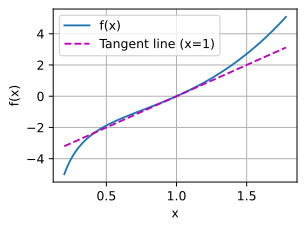
\includegraphics[width=0.6\textwidth]{Images/4_6.png}
    \end{center}
	\end{itemize}
\item Find the gradient of the function $f(x) = ||x||_2$? What happens for $x = 0$?
	\begin{itemize}
	\item Note that if $x = (x_1, \dots, x_n)$ then $g(x) := f(x)^2 = ||x||_2^2 = \sum_{i = 1}^n x_i^2$. It follows that for $x \neq 0$ the corresponding partial derivates are simply given by
	$$
	\frac{\partial}{\partial x_j} f(x)^2 = \frac{\partial}{\partial x_j} \sum_{i = 1}^n x_i^2 = 2 x_i.
	$$
	This shows that $\nabla g(x) = 2 x$. Furthermore $\frac{\partial}{\partial x_j} g(x) = \frac{\partial}{\partial x_j} f(x)^2 = 2 \frac{\partial f}{\partial x_j} \cdot f(x)$. With that we can calculate
	$$
	2x = 2 f(x) \nabla f \iff \nabla f = \frac{x}{f(x)} = x / ||x||.
	$$
	Note that this construction breaks down at $x = 0$ as we would divide by $0$. But this is not surprising because $x \mapsto \sqrt{x}$ is not differentiable at $0$ and $f(x) = \sqrt{g(x)}$.
	\end{itemize}
\item Can you write out the chain rule for the case where $u = f(x, y, z)$ and $x = x(a, b), y = y(a, b)$ and $z = z(a, b)$?
	\begin{itemize}
	\item We can write $u(a, b) = f(x(a, b), y(a, b), z(a, b))$ and with that
	$$
	\frac{\partial}{\partial a} u(a, b) = \frac{\partial f}{\partial x}(\dots) \cdot \frac{\partial x}{\partial a} + \frac{\partial f}{\partial y}(\dots) \cdot \frac{\partial y}{\partial a} + \frac{\partial f}{\partial z}(\dots) \cdot \frac{\partial z}{\partial a},
	$$
	which can be expressed as
	$$
	(\nabla f)(x(a, b), y(a, b), z(a, b)) \cdot \nabla_a (x, y, z).
	$$
	Similiarly once can show taht
	$$
	(\nabla f)(x(a, b), y(a, b), z(a, b)) \cdot \nabla_b (x, y, z).
	$$
	With that it follows that
	$$
	\nabla u(a, b) = (\nabla f, \nabla f)^t \cdot (D(x, y, z)).
	$$
	\end{itemize}
\item Given a function $f(x)$ that is invertible, compute the derivative of its inverse $f^{-1}(x)$. Here we have that $f^{-1}(f(x)) = x$ and conversely $f(f^{-1}(y)) = y$. Hint: Use these properties in your derivation.
	\begin{itemize}
		\item We can calculate
		$$
		1 = \frac{\partial}{\partial x} x = \frac{\partial}{\partial x} f^{-1}(f(x)) = (f^{-1})'(f(x)) f'(x),
		$$
		which can be rewritten as
		$$
		(f^{-1})'(f(x)) = \frac{1}{f'(x)}.
		$$
		If we write $y = f(x)$ this becomes
		$$
		(f^{-1})'(y) = \frac{1}{f'(x)}.
		$$
	\end{itemize}
\end{enumerate}

\subsection{Automatic Differentiation}
\begin{enumerate}
\item Why is the second derivative much more expensive to compute than the first derivative?
	\begin{itemize}
		The derivative can be approximated by sampling two points, the second derivative needs more points. If we consider the second derivative as the derivative of the derivative then we need to sample two points at each of the original sampling points, which more than doubles the workload. Note that the second derivative is the average rate of change of the rate of change of the two sample points, symbolically:
		$$
		f'(x_0) \sim f(x_0 + \varepsilon) - f(x_0 - \varepsilon)
		$$
		and
		\begin{align*}
		f'(x_0 + \varepsilon) = f(x_0 + 2\varepsilon) - f(x_0),&&f'(x_0 - \varepsilon) = f(x_0) - f(x_0 - 2\varepsilon).
		\end{align*}
		From this it can be seen that the second derivative can be expressed as
		\begin{align*}
		f''(x_0) &= f'(x_0 + \varepsilon) - f'(x_0 - \varepsilon) \\
		&= f(x_0 + 2\varepsilon) - f(x_0) - (f(x_0) - f(x_0 - 2\varepsilon)) \\
		&= f(x_0 + 2\varepsilon) - 2f(x_0) + f(x_0 - 2\varepsilon)).
		\end{align*}
		There are much better choice for sampling points to get faster numerical convergence, but this is beyond the scope of what we're doing here. 
	\end{itemize}
\item After running the function for backpropagation, immediately run it again and see what happens. Why?
\item In the control flow example where we calculate the derivative of d with respect to a, what would happen if we changed the variable a to a random vector or a matrix? At this point, the result of the calculation f(a) is no longer a scalar. What happens to the result? How do we analyze this?
\item Let $f(x) = \sin(x)$. Plot the graph of $f$ and its derivative $f'$. Do not exploit the fact that $f'(x) = \cos(x)$ but rather use automatic differentiation to get the result.
\item Let $f(x) = ((\log x^2) \cdot \sin x) + x^{-1}$. Write out a dependency graph tracing results from $x$ to $f(x)$.
\item Use the chain rule to compute the derivative $f'$ of the aforementioned function, placing each term on the dependency graph that you constructed previously.
\item Given the graph and the intermediate derivative results, you have a number of options when computing the gradient. Evaluate the result once starting from $x$ to $f$ and once from $f$ tracing back to $x$. The path from $x$ to $f$ is commonly known as \textit{forward differentiation}, whereas the path from $f$ to $x$ is known as \textit{backward differentiation}.
\item When might you want to use forward differentiation and when backward differentiation? Hint: consider the amount of intermediate data needed, the ability to parallelize steps, and the size of matrices and vectors involved.
\end{enumerate}

\subsection{Probability and Statistics}
This might be a bit too technical for the course, but to remind myself of the background. Let $(\Omega, \mathcal{A}, P)$ be a probability space, this is a measure space (i.e. $\Omega$ is some set, $\mathcal{A}$ is a sigma algebra on $\Omega$ and $P$ is a measure, i.e. a $\sigma$-additive function $P : \mathcal{A} \rightarrow [0, +\infty)$ which satisfies $P(\emptyset) = 0$), where the measure is a probability function, i.e. $P(\Omega) = 1$. Recall that this means that probability theory is only interested in the theory of finite measures.

A random variable is a measureable function $X : \Omega \rightarrow \mathbb{R}$. We call the elements of the sigma algebra an event (and the sigma-algebra itself the event space) and the elements of $\Omega$ a sample (and $\Omega$ itself a sample space). The expression
$$
P\left(\lim_{n \rightarrow \infty} X_n = \alpha\right) = p
$$
is simply shorthand for
$$
P\left(\{\omega \in \Omega : \lim_{n \rightarrow \infty} X_n(\omega) = \alpha\}\right) = p.
$$
\begin{enumerate}
	\item Give an example where observing more data can reduce the amount of uncertainty about the outcome to an arbitrarily low level.
	\begin{itemize}
		\item Consider flipping a weighted coin, whose probability to land on heads is given by $p_H \in (0, 1)$. Let $(X_i)_{i \in \mathbb{N}}$ be a sequence of random variables where $X_i \in \{0, 1\}$ and is $1$ if the $i$th flip landed on heads. Counting the outcome of the first $n$ flips yields the random variable
		$$
		\tilde{X}_n := \sum_{i}^n X_i.
		$$
		Note that
		$$
		P\left(\lim_{n \rightarrow \infty} \frac{\tilde{X}_n}{n} \neq p_H\right) = 0,
		$$
		or if we consider the running average $Y_n := \frac{1}{n} \tilde{X}_n$ this can be expressed as
		$$
		P\left(\lim_{n \rightarrow \infty} Y_n = p_H\right) = 1.
		$$
	\end{itemize}

	\item Give an example where observing more data will only reduce the amount of uncertainty up to a point and then no further. Explain why this is the case and where you expect this point to occur.
	\begin{itemize}
		\item Sticking to the same example as before, flipping a fair coin. If the question is what is the probability that the coin is fair, we get a convergence to $100\%$. But if we instead ask what is the probability that the next flip will be heads we can only have a certainty of $50\%$ that it will be heads. If $p$ denotes the probability of heads, we can establish this value arbitrarily close, but the probability of getting heads will still be $p$. This uncertainty is inherent to the system. Using the notation of the book, this is an example of aleatoric uncertainty, while the actual value of $p$ is epistemic uncertainty.
	\end{itemize}
	\item We empirically demonstrated convergence to the mean for the toss of a coin. Calculate the variance of the estimate of the probability that we see a head after drawing $n$ samples.
		\begin{itemize}
			\item Let $X_i \in \{0, 1\}$ denote if the $i$th flip landed on head and consider 
			$$
			\tilde{X}_n := \sum_{i = 1}^n X_i.
			$$
			We are interested in $P(\tilde{X}_n \geq 1)$. Note that for $k \in {0, \dots, n}$ the statement $\tilde{X}_n = k$ is equivalent to there being exactly $k$ heads, which means we have $k$ heads and $n - k$ tails. Denote by $p$ the probability of getting heads, then flipping $k$ heads and $n - k$ tails has a probability of
			$$
			p^k (1 - p)^{n - k}
			$$
			and because the order of those doesn't matter we have to multiply this with the number of permutations, i.e., we are interested in how many arrangements there are to distribute $k$ (or equivalently $n - k$) elements in $n$ slots. This is exactly the binomial coefficient
			$$
			\binom{n}{k} = \frac{n!}{k! (n - k)!}.
			$$
			In total this means
			$$
			P(\tilde{X}_n = k) = \binom{n}{k} p^k (1 - p)^{n - k}.
			$$

			Looking back on it now, I just realized that the $X_i$ are all independent as such
			$$
			E[\tilde{X}_n] = E\left[\sum_{i = 1}^n X_i\right] = \sum_{i = 1}^n E[X_i] = \sum_{i = 1}^n p = np.
			$$

			Alternatively the expected value of $\tilde{X}_n$ can then be calculated directly as
			$$
			\begin{aligned}
			E[\tilde{X}_n] &= \sum_{k = 0}^n kP(\tilde{X}_n = k) \\
			&= \sum_{k = 0}^n k \binom{n}{k} p^k (1 - p)^{n - k} \\
			&= \sum_{k = 0}^n k \binom{n}{k} p^k (1 - p)^{n - k}.
			\end{aligned}
			$$
			This can be explicitly calculated to be $np$, we're only going to prove the case where $p = 1 - p = 0.5$, in that case
			$$
			\begin{aligned}
			E[\tilde{X}_n] &= \sum_{k = 0}^n k \binom{n}{k} 2^{-n}
			&= 2^{-n} \sum_{k = 0}^n k \binom{n}{k} \\
			&\overset{*}{=} 2^{-n} 2^{n - 1} = n / 2 = pn.
			\end{aligned}
			$$
			What remains to be shown is that $(*)$ holds. This can be done inductively, it obviously holds for $n = 1$. Now suppose the identity holds for some $n \in \mathbb{N}$, then
			$$
			\sum_{k = 0}^{n + 1} k \binom{n + 1}{k} = (n + 1) + \sum_{k = 0}^n k \binom{n + 1}{k},
			$$
			using Pascal's triangle equality we can write
			$$
			\binom{n + 1}{k} = \binom{n}{k} + \binom{n}{k - 1}.
			$$
			With this we can then calculate
			$$
			\begin{aligned}
			\sum_{k = 0}^{n + 1} k \binom{n + 1}{k} &= (n + 1) + \sum_{k = 0}^n k \binom{n + 1}{k} \\
			&= (n + 1) + \sum_{k = 0}^n k \left[ \binom{n}{k} + \binom{n}{k - 1} \right] \\
			&= (n + 1) + \sum_{k = 0}^n k \binom{n}{k} + \sum_{k = 0}^n k \binom{n}{k - 1} \\
			&= (n + 1) + \sum_{k = 0}^n k \binom{n}{k} + \sum_{k = 0}^{n - 1} (k + 1) \binom{n}{k} \\
			&= (n + 1) + \sum_{k = 0}^n k \binom{n}{k} + \sum_{k = 0}^{n - 1} k \binom{n}{k} + \sum_{k = 0}^{n - 1} \binom{n}{k} \\
			&= (n + 1) + \sum_{k = 0}^n k \binom{n}{k} + \sum_{k = 0}^n k \binom{n}{k} + \sum_{k = 0}^{n - 1} \binom{n}{k} - n \\
			&= 2 \sum_{k = 0}^n k \binom{n}{k} - n + \sum_{k = 0}^n \binom{n}{k} - 1.
			\end{aligned}
			$$
			Applying the well-known identity
			$$
			\sum_{k = 0}^n \binom{n}{k} = 2^n
			$$
			and the induction hypothesis to this yields
			$$
			2 (2^{n - 1}) + 2^n = 2^{n + 1}.
			$$
			By induction it then follows that for all $n \in \mathbb{N}$ the identity
			$$
			\sum_{k = 0}^n k \binom{n}{k} = 2^n
			$$
			holds.
			\item Just as for the expected value
			$$
			\operatorname{Var}[\tilde{X}_n] = \sum_{i = 1}^n \operatorname{Var}[X_i] = np(1 - p).
			$$
		\end{itemize}
		\begin{enumerate}
			\item How does the variance scale with the number of observations?
				\begin{itemize}
					\item It scales linearly.
				\end{itemize}
			\item Use Chebyshev's inequality to bound the deviation from the expectation.
				\begin{itemize}
					\item For $p = 1/2$ the mean is $\mu = n / 2$ and the standard deviation is $\sigma = \sqrt{n} / 2$. Applying Chebychev's inequality with these values and $k > 0$ yields
					$$
					P\left(\left|\tilde{X}_n - \frac{n}{2}\right| \geq k \frac{\sqrt{n}}{2}\right) \leq \frac{1}{k^2}.
					$$
					For example for $n = 16$ and $k = 2$ this becomes
					$$
					P(|\tilde{X}_{16} - 8| \geq 4) \leq \frac{1}{4},
					$$
					inverting this statement then proves that $P(6 \leq \tilde{X}_{16} \leq 10) \geq \frac{3}{4}$, i.e., there is a more than $75\%$ chance that on flipping $16$ (fair) coins we have at least $6$ and at most $10$ heads.
				\end{itemize}
			\item How does it relate to the central limit theorem?
				\begin{itemize}
					\item $$\lim_{n \rightarrow \infty} \frac{\tilde{X}_n - n / 2}{\sqrt{n} / 2}$$ converges to the standard normal distribution.
				\end{itemize}
		\end{enumerate}
	\item Assume that we draw samples from a probability distribution with zero mean and unit variance. Compute the averages
	$$
	z_m = m^{-1} \sum_{i = 1}^m X_i.
	$$
	Can we apply Chebychev's inequality for every $z_m$ independently? Why not?
		\begin{itemize}
			\item I'll assume we're talking about $X_i$ with finite amounts of values. The $X_i$ are independent so
			$$
			E[z_m] = E[m^{-1}\sum_i^m X_i] = m^{-1} \sum_{i = 1}^m \underbrace{E[X_i]}_{=\ 0} = 0.
			$$
			No, we can't apply Chebychev's inequality independently because $z_{m + 1} = z_m + X_{m + 1}$ as such $z_m$ and $z_{m + 1}$ are not independent.
		\end{itemize}
	\item Given two events with probability $P(\mathcal{A})$ and $P(\mathcal{B})$ compute upper and lower bounds on $P(\mathcal{A} \cup \mathcal{B})$ and $P(\mathcal{A} \cap \mathcal{B})$. Hint: graph the situation using a Venn diagram.
		\begin{itemize}
			\item Using a Venn diagram we can immediately see that
			$$
			\max\{P(A), P(B) \} \leq P(A \cup B) = P(A) + P(B) - P(A \cap B) \leq P(A) + P(B),
			$$
			and
			$$
			P(A) + P(B) - 1 \leq P(A \cap B) \leq \min\{P(A), P(B)\}
			$$
			holds.
		\end{itemize}
	\item Assume that we have a sequence of random variables, say $A, B$, and $C$, where $B$ only depends on $A$, and $C$ only depends on $B$, can you simplify the joint probability $P(A, B, C)$? Hint: this is a Markov chain.
		\begin{itemize}
			\item Note that $P(A, B)$ is just shorthand for $P(A \cap B)$.
			\begin{align*}
			P(A, B, C) &= P(A|B, C) P(B, C) \\
			&= P(A|B) P(B, C) \\
			&= P(A|B) P(B|C) P(C)
			\end{align*}
			where we have used (2.6.1) from the book, as well as because $A$ and $C$ are independent it follows that $P(A|B, C) = P(A|B)$. This can be expressed more generally, if we have a collection of random variables $X_i$ such that
			$$
			P(X_{i + 1} | X_i, X_{i - 1}, \dots, X_1) = P(X_{i + 1}| X_i),
			$$
			i.e. $X_{i + 1}$ only "remembers" the previous variable then
			$$
			P(X_n, \dots, X_1) = P(X_n|X_{n - 1})P(X_{n - 2}|X_{n - 3})\cdot \dots \cdot P(X_1|X_0)P(X_0).
			$$
		\end{itemize}
	\item In Section 2.6.5, assume that the outcomes of the two tests are not independent. In particular assume that either test on its own has a false positive rate of $10\%$ and a false negative rate of $1\%$. That is, assume that
	$$
	P(D = 1 | H = 0) = 0.1,
	$$
	and that
	$$
	P(D_1, D_2 | H = 1) = 0.02.
	$$
	\begin{enumerate}
		\item Work out the joint probability table for $D_1$ and $D_2$ given $H = 0$ based on the information you have so far.
			\begin{itemize}
				\item
					\begin{center}
						\begin{tabular}{|c|c|c|} \hline
						Conditional Probability & $H = 1$ & b \\ \hline
						& a & b \\ \hline
						\end{tabular}
					\end{center}
			\end{itemize}
		\item Derive the probability of the patient being positive $(H = 1)$ after one test returns positive. You can assume the same baseline probability $P(H = 1) = 0.0015$ as before.
		\item Derive the probability of the patient being positive $(H = 1)$ and both tests return positive.
	\end{enumerate}
	\item Assume that you are an asset manager for an investment bank and you have a choice of stocks $s_i$ to invest in. Your portfolio needs to add up to $1$ with weights $\alpha_i$ for each stock. The stocks have an average return $\mu = E_{s \sim P}[s]$ and covariance $\Sigma = \operatorname{Cov}_{s \sim P}[s]$.
		\begin{enumerate}
			\item Compute the expected return for a given portfolio $\alpha$.
				\begin{itemize}
					\item A portfolio is a choice of weights $(\alpha_1, \dots, \alpha_n)$ where $\alpha_i \geq 0$ and $\sum_{i = 1}^n \alpha_i = 1$. The expected return of $s_i$ is denoted by $\mu$ and the expected return of the portfolio is
					$$
					\sum_{i = 1}^n \alpha_i \mu_i.
					$$
				\end{itemize}
			\item If you wanted to maximize the return of the portfolio, how should you choose your investment?
				\begin{itemize}
					\item Let $j = \operatorname{arg} \max_{1 \leq i \leq n} \mu_i$ then the portfolio $\alpha^{(j)} := s_j$ has expected return of $\mu_j$, which is an upper bound on the returns of all portfolios:
					$$
					\sum_{i = 1}^n \alpha_i \mu_i \leq \sum_{i = 1}^n \alpha_i \max_i \mu_i = \left(\sum_{i = 1}^n \alpha_i\right) \max_i \mu_i = \mu_j.
					$$
				\end{itemize}
			\item Compute the variance of the portfolio.
				\begin{itemize}
					\item Recall that the variance of $x \mapsto v^t x, v = (\alpha_1, \dots, \alpha_n)$ can be expressed by using the covariance matrix as follows:
					$$
					\operatorname{Var}(v) = v^t \Sigma v.
					$$
				\end{itemize}
			\item Formulate an optimization problem of maximizing the return while keeping the variance constrained to an upper bound. This is the Nobel-Prize winning Markovitz portfolio (Mangram, 2013). To solve it you will need a quadratic programming solver, something way beyond the scope of this book.
				\begin{itemize}
					\item Let $V_0 > 0$ be our upper bound on the variance. We want to maximize $\sum_{i = 1}^n \alpha_i \mu_i$ such that
					$$
					(\alpha_1, \dots, \alpha_n) \Sigma \begin{pmatrix} \alpha_1 \\ \alpha_2 \\ \vdots \\ \alpha_n \end{pmatrix} \leq V_0.
					$$
				\end{itemize}
		\end{enumerate}
\end{enumerate}

\newpage
\section{Linear Neural Networks for Regression}
\subsection{Linear Regression}
\begin{enumerate}[label=\arabic*.]
\item Assume that we have some data $x_1, \dots x_n \in \mathbb{R}$. Our goal is to find a constant $b$ such that $\sum_i (y_i - b)^2$ is minimized.
	\begin{enumerate}[label=\arabic*.]
	\item Find an analytic solution for the optimal value of $b$.
		\begin{itemize}
			\item Consider the function
			\begin{align*}
			f : \mathbb{R}^n \times \mathbb{R} &\rightarrow [0, \infty) \\
			(y, b) &\mapsto \sum_{i = 1}^n (y_i - b)^2.
			\end{align*}
			For fixed $y \in \mathbb{R}^n$ we want to solve the following minimization problem, find $b^*_y$ such that
			$$
			\min_{b \in \mathbb{R}} f(y, b) = f(y, b^*_y)
			$$
			\begin{align*}
			\sum_{i = 1}^n (y_i - b)^2 = \sum_{i = 1}^n (y_i^2 - 2y_i b + b^2) = \sum_{i = 1}^n y_i^2 \underbrace{- 2 b \underline{y} + b^2}_{=: g(b)}
			\end{align*}
			As such we are looking for the minimum of $g(b)$. Obviously $g$ is continuously differentiable and we can calculate
			$$
			g'(b) = -2 \sum_{i = 1}^n y_i + 2b = 2 (b - \sum_{i = 1}^n y_i) = 0
			$$
			meaning that $b^* = \sum_{i = 1}^n y_i$ is the (unique!) solution to our minimization problem.
		\end{itemize}
	\item How does this problem and its solution relate to the normal distribution?
	\item What if we change the loss from
		\begin{equation*}
		\sum_i (x_i - b)^2
		\end{equation*}
		to
		\begin{equation*}
		\sum_i |x_i - b|?
		\end{equation*}
		Can you find the optimal solution for $b$?
			\begin{itemize}
				\item Consider $b' := \overline{y}$, our new "linear" error function can be written as follows:
				\begin{align*}
				\sum_{i = 1}^n |y_i - b| &= \sum_{i = 1, y_i < \overline{y}}^n |y_i - \overline{y}| + \sum_{i = 1, y_i > \overline{y}}^n |y_i - \overline{y}| \\
				&= \sum_{i = 1, y_i < \overline{y}}^n \overline{y} - y_i + \sum_{i = 1, y_i > \overline{y}}^n y_i - \overline{y}
				\end{align*}
			\end{itemize}
	\end{enumerate}
\item Prove that the affine functions that can be expressed by $y = Wx + b$ are equivalent to linear functions on $(x, 1)$.
	\begin{itemize}
		\item Consider $C := (w, 1)$ then $C^t(x, b) = (w^t|1)$ and
		$$
		\begin{pmatrix}
		w & 1
		\end{pmatrix}
		\begin{pmatrix}
		x \\ b
		\end{pmatrix} = 
		wx + b
		$$
	\end{itemize}
\item Assume that you want to find quadratic functions of $y$, i.e.,
	$$
	y = Wx^2 + b.
	$$
	How would you formulate this in a deep network?
\item Recall that one of the conditions for the linear regression problem to be solvable was that the design matrix $X$ has full rank.
	\begin{enumerate}[label=\arabic*.]
	\item What happens if this is not the case?
	\item How could you fix it? What happens if you add a small amount of coordinate-wise independent Gaussian noise to all entries of $X$?
	\item What is the expected value of the design matrix $X^tX$ in this case?
	\item What happens with stochastic gradient descent when $X^tX$ does not have full rank?
	\end{enumerate}
\item Assume that the noise model governing the additive noise $e_i$ is the exponential distribution. That is, $p(e_i) = \lambda e^{-\lambda e_i}$.
	\begin{enumerate}[label=\arabic*.]
	\item Write out the negative log-likelihood of the data under the model $p(e_i)$.
	\item Can you find a closed form solution?
	\item Suggest a minibatch stochastic gradient descent algorithm to solve this problem. What could possibly go wrong (hint: what happens near the stationary point as we keep on updating the parameters)? Can you fix this?
	\end{enumerate}
\item Assume that we want to design a neural network with two layers by composing two linear layers. That is, the output of the first layer becomes the input of the second layer. Why would such a naive composition not work?
\item What happens if you want to use regression for realistic price estimation of houses or stock prices?
	\begin{enumerate}[label=\arabic*.]
	\item Show that the additive Gaussian noise assumption is not appropriate. Hint: can we have negative prices? What about fluctuations?
	\item Why would regression to the logarithm of the price be much better, i.e., $y = \log \operatorname{price}$?
	\item What do you need to worry about when dealing with pennystock, i.e., stock with very low prices? Hint: can you trade at all possible prices? Why is this a bigger problem for cheap stock?
	\item For more information review the celebrated Black-Scholes model for option pricing (Black and Scholes, 1973).
	\end{enumerate}
\item Suppose we want to use regression to estimate the number of apples sold in a grocery store.
	\begin{enumerate}[label=\arabic*.]
	\item What are the problems with a Gaussian additive noise model? Hint: you are selling apples, not oil.
	\item The Poisson distribution captures distributions over counts. It is given by $P(k; \lambda) = \frac{e^{-\lambda} \lambda^k}{k!}$. Here $\lambda$ is the rate function and $k$ is the number of events you see. Prove that $\lambda$ is the expected value of counts $k$.
	\item Design a loss function associated with the Poisson distribution.
	\item Design a loss function for estimating $\log \lambda$ instead.
	\end{enumerate}
\end{enumerate}

\newpage
\setcounter{section}{22}
\section{Appendix: Mathematics for Deep Learning}
\subsection{Geometry and Linear Algebraic Operations}
\begin{enumerate}
\item What is the angle between
$$
\begin{aligned}
\vec v_1 = \begin{pmatrix} 1 \\ 0 \\ -1 \\ 2 \end{pmatrix},&& \vec{v_2} = \begin{pmatrix} 3 \\ 1 \\ 0 \\ 1 \end{pmatrix}?
\end{aligned}
$$
	\begin{itemize}
		\item We know that
		$$
			\cos(\alpha) = \frac{\vec{v_1} \cdot \vec{v_2}}{||\vec{v_1}|| ||\vec{v_2}||}
		$$
		We can calculate $||\vec{v_1}|| = \sqrt{6}, ||\vec{v_2}|| =  \sqrt{11}$ and $\vec{v_1} \cdot \vec{v_2} = 5$. From this we see that
		$$
		\cos{\alpha} = \frac{5}{\sqrt{66}} = 0.9078
		$$
		which in degrees is $51.02^\circ$.
	\end{itemize}
\item True or false: $\begin{pmatrix}1 & 2 \\ 0 & 1\end{pmatrix}$ and $\begin{pmatrix}1 & -2 \\ 0 & 1 \end{pmatrix}$ are inverses of one another?
	\begin{itemize}
		\item This is true, this can be shown either by multiplying them or noting that the determinant of the first matrix is $1$ and using the identity
		$$
		\begin{pmatrix}
		a & b \\
		c & d \\
		\end{pmatrix}^{-1} =
		\frac{1}{ad - bc}
		\begin{pmatrix}
		d & -b \\
		-c & a \\
		\end{pmatrix}
		$$
	\end{itemize}
\item Suppose that we draw a shape in the plane with area $100m^2$. What is the area after transforming the figure by the matrix $$ \begin{pmatrix} 2 & 3\\ 1 & 2 \end{pmatrix}. $$
	\begin{itemize}
		\item It is exactly scaled by the determinant, which is $1$, as such the new area is also $100m^2$.
	\end{itemize}
\item Which of the following sets of vectors are linearly independent?
$$
\begin{aligned}
\left\{\begin{pmatrix} 1 \\ 0 \\ -1\end{pmatrix}, \begin{pmatrix} 2 \\ 1 \\ -1 \end{pmatrix}, \begin{pmatrix} 3 \\ 1 \\ 1 \end{pmatrix}\right\},&&\left\{\begin{pmatrix} 3 \\ 1 \\ 1\end{pmatrix}, \begin{pmatrix} 1 \\ 1 \\ 1 \end{pmatrix}, \begin{pmatrix} 0 \\ 0 \\ 0 \end{pmatrix}\right\}, &&\left\{\begin{pmatrix} 1 \\ 1 \\ 0\end{pmatrix}, \begin{pmatrix} 0 \\ 1 \\ -1 \end{pmatrix}, \begin{pmatrix} 1 \\ 0 \\ 1 \end{pmatrix}\right\}
\end{aligned}
$$
\item Suppose that you have a matrix written as $A = \begin{pmatrix} c \\ d \end{pmatrix} \cdot \begin{pmatrix} a & b \end{pmatrix}$ for some choice of values $a, b, c,$ and $d$. True or false: the determinant of such a matrix is always $0$?
	\begin{itemize}
		\item Yes it is, this is pretty much exactly what it means for the matrix to be rank $1$ (or $0$ if $a = b = c = d$). If $a = 0$ then the matrix can't be rank $2$ and otherwise we can remove the second column by adding $d / a$ times the first colum onto the second. This leaves the determinant unchanged and the new matrix has an empty column.
	\end{itemize}
\item The vectors $e_1 = \begin{pmatrix} 1 \\ 0 \end{pmatrix}$ and $e_2 = \begin{pmatrix} 0 \\ 1 \end{pmatrix}$ are orthogonal. What is the condition on a matrix $A$ so that $Ae_1$ and $A_2$ are orthogonal?
	\begin{itemize}
		\item Suppose
		$$
		A = \begin{pmatrix} a & b \\ c & d \end{pmatrix}
		$$
		then $Ae_1 = (a, c)$ and $Ae_2 = (b, d)$. As such $A_e1 \cdot Ae_2 = ab + cd$, for this to be zero we need to have $ab = -cd$. If $a = 0$ this means that $c$ or $d$ has to be zero. Otherwise we have $b = - \frac{cd}{a}$. AS such $Ae_1$ and $Ae_2$ are orthogonal either if $a = 0$ or the matrix is of the form
		$$
		A = \begin{pmatrix} a & - \frac{cd}{a} \\ c & d \end{pmatrix}.
		$$
	\end{itemize}
\item How can you write $\operatorname{tr}(A^4)$ in Einstein notation for an arbitrary matrix $A$?
	\begin{itemize}
		\item First note that we can express the trace as follows:
		$$
		\begin{aligned}
		\operatorname{tr}(A^4) &= \sum_i A^4_{ii} \\
		&= \sum_i \sum_j A_{ij} A^3_{ji} \\
		&= \sum_i \sum_j \sum_k A_{ij} A_{jk} A^2_{ki} \\
		&= \sum_i \sum_j \sum_k \sum_r A_{ij} A_{jk} A_{kr} A_{rk} A_{ki}.
		\end{aligned}
		$$
		Using Einstein notation this then becomes
		$$
		\operatorname{tr}(A^4) = A_{ij} A^j_k A^k_r A^r_k A^{ki}.
		$$
	\end{itemize}
\end{enumerate}

\subsection{Eigendecompositions}
\begin{enumerate}
\item What are the eigenvalues and eigenvectors of
$$
A = \begin{pmatrix} 2 & 1 \\ 1 & 2 \end{pmatrix}
$$
	\begin{itemize}
		\item Recall that $\chi_A(x) = x^2 + \operatorname{tr}(A)x + \det(A) = x^2 + 4x + 3 = (x + 3)(x + 1)$, so the eigenvalues are $-3$ and $-1$.
	\end{itemize}
\item What are the eigenvalues and eigenvectors of the following matrix, and what is strange about this example compared to the previous one?
$$
\begin{pmatrix}
2 & 1 \\
0 & 2
\end{pmatrix}
$$
	\begin{itemize}
		\item Sidenote: This is the Jordan block $J_2(2)$. Here the trace and the determinant are the same thing so the characteristic polynomial is $\chi_A(x) = x^2 + 4x + 4 = (x + 2)^2$ so we have the eigenvalue $-2$ with multiplicity $2$.
	\end{itemize}
\item Without computing the eigenvalues, is it possible that the smallest eigenvalue of the following matrix is less that $0.5$? Note: this problem can be done in your head.
$$
\begin{pmatrix}
$3.0$ & $0.1$ & $0.3$ & $1.0$ \\
$0.1$ & $1.0$ & $0.1$ & $0.2$ \\
$0.3$ & $0.1$ & $5.0$ & $0.0$ \\
$1.0$ & $0.2$ & $0.0$ & $1.8$
\end{pmatrix}.
$$
	\begin{itemize}
		\item Recall the discussion on the Gershgorin Circle Theorem. $(r_1, r_2, r_3, r_4) = (1.4, 0.4, 0.4, 1.2)$ as such the corresponding eigenvalues all lie within the rances $[a_{ii} - r_i, a_{ii} + r_i]$, i.e. within
		$$
		[1.6, 4.4] \cup [0.6, 1.4] \cup [4.6, 5.4] \cup [0.6, 3] = [0.6, 4.4] \cup [4.6, 5.4]
		$$
		and $(-\inf, 0.5)$ does not intersect this set. As such there can't be any eigenvalue $\lambda < 0.5$.
	\end{itemize}
\end{enumerate}

\subsection{Single Variable Calculus}
\begin{enumerate}
	\item What is the derivative of $f_1(x) = x^3 - 4x + 1$?
		\begin{itemize}
			\item $f_1'(x) = 3x^2 - 4$.
		\end{itemize}
	\item What is the derivative of $f_2(x) = \log\left( \frac{1}{x} \right)$?
		\begin{itemize}
			\item Note that $f_2(x) = \log\left(\frac{1}{x}\right) = \log(x^{-1}) = - \log(x)$ so the derivative is $f_2'(x) = - \frac{1}{x}$.
		\end{itemize}
	\item True or False: If $f_3'(x) = 0$ then $f_3$ has a maximum or minimum at $x$?
		\begin{itemize}
			\item Wrong, for example if $f''_3(0) = 0$ then we have a saddle point. This is for example the case when $f_3(x) = x^3$.
		\end{itemize}
	\item Where is the minimum of $f_4(x) = x \log(x)$ for $x \geq 0$ (where we assume that $f_4$ takes the limiting value of $0$ at $f_4(0)$)?
		\begin{itemize}
			\item First note that for $x \in (0, 1)$ we have $f_4(x) < 0$ and for $x \in \{0\} \cup [1, \infty)$ we have $f_4(x) \geq 0$ so the minimum has to be attained by some $x \in (0, 1)$. Also note that $f_4$ is a smooth map, $[0, 1]$ is compact so this minimum is actually attained. To determine the minimum we want to solve $f_4'(x) = \log(x) + 1 = 0$:
			$$
			\begin{aligned}
			&& \log(x) + 1 &= 0 \\
			\iff\ && \log(x) &= -1 \\
			\iff\ && -\log(x) &= 1 \\
			\iff\ && \log(x^{-1}) &= 1 \\
			\iff\ &&  x^{-1} &= e \\
			\iff\ && x &= \frac{1}{e}.
			\end{aligned}
			$$
		\end{itemize}
\end{enumerate}

\end{document}